\documentclass[ %
  graybox       %
 ,envcountchap  %
 ,sectrefs      %
% ,footinfo      %
% ,graphics      %
%,referee
]{svmono}
% Native packages
\usepackage{mathptmx}
\usepackage{helvet}
\usepackage{courier}
\usepackage{type1cm}
\usepackage{makeidx}		    % allows index generation
\usepackage{graphicx}		    % standard LaTeX graphics tool
\usepackage{multicol} 		    % used for the two-column index
\usepackage[bottom]{footmisc}	% places footnotes at page bottom
% User packages
\usepackage{natbib}
\usepackage{lipsum}
\usepackage{placeins}
\usepackage{multirow}			% added by Matt
%\makeindex             		% used for the subject index: please use the style svind.ist with your makeindex program
\begin{document}
\author{Matthew James Green and Kees van Deemter}
\title{Vagueness \& Rationality}
\subtitle{The Elusive Benefits of Vagueness: the Evidence So Far}
\date{}
\maketitle
\frontmatter
\tableofcontents
\mainmatter
\chapter{The Elusive Benefits of Vagueness: Evidence from Experiments}\label{chapterlabel}
Much of everyday language is vague, even in situations where vagueness could have been avoided (i.e., where vagueness is used ``strategically''). Yet the benefits of vagueness for hearers and readers are proving to be elusive. We discuss a range of earlier controlled experiments with human participants, and we report on a new series of experiments that we conducted in recent years. These experiments, which focus on vague expressions that are part of referential noun phrases, aim to separate the utility of vagueness (as defined by the existence of borderline cases) from the utility of other factors that tend to co-occur with vagueness. Having presented the evidence, we argue that the evidence supports a view where the benefits that vague terms exert are due to other influences, and not to vagueness itself.

\section{Introduction}\label{introduction}In most academic use, the word `vagueness' has a specific meaning. Keefe and Smith, for example, state ``vague predicates have borderline cases, have fuzzy boundaries, and are susceptible to sorites paradoxes'' \citep[p.~4]{keefe1997vagueness}, also \citet{EgreKlinedinst}.  The crucial criterion is the existence of borderline cases: ``a word is precise if it describes a well-defined set of objects. By contrast, a word is vague if it is not precise'' \citet[p.~1]{lipmanvague}. A typical example is the word ``tall'', as applied to people for example, because here is no precise, known height which separates those who are tall from those who are not. The crucial point is that ``tall'' admits borderline cases (i.e., people who may or may not count as tall), which are the hallmark of vagueness as we use the term.

Linguists, philosophers of language, and more recently game theorists, have asked why natural languages contain so many vague expressions \citet{Lipman:2000fk, lipmanvague}, which are
often used even in situations where the speaker could have used an expression that is not vague (i.e., crisp); in these situations we say that vagueness is used \emph{strategically}. By introducing borderline cases, these expressions create potential misunderstandings, thereby creating ``a worldwide several-thousand year efficiency loss'' \citet[][p.~1]{lipmanvague}. Lipman explains the point by means of a scenario in which a speaker describes a person to a hearer, who needs to identify that person in the arrivals hall of of an airport. In such a scenario, a precise description of the person's height (e.g., ``The person's height is 187.96 cm'') would be more useful than a vague one (``The person is tall''). Lipman uses this scenario to explain why standard game theory models of communication \citep[e.g.,][]{Crawford:1982lr} predict that, under certain conditions, a crisp act of communication will always have more utility than a vague act that communicates the same state of affairs. 

Lipman argued that the efficiency loss resulting from vague expressions would be unlikely to have arisen unless there are advantages as well as disadvantages associated with vague expressions. Lipman asked, essentially, what these advantages might be. Several tentative answers to Lipman's question have been offered \citep[see][]{van2009utility, vanDeemterBook}. One of the most promising answers appears to be the idea that vague expressions are easier to process, by a speaker and/or a hearer, than expressions that are not vague (i.e., crisp) \citep[e.g.,][]{lipmanvague,De-Jaegher:2003lr,vanrooij2003lr}. For example, \citeauthor{lipmanvague} writes: ``For the listener, information which is too specific may require more effort to analyze'' (\citeyear[][p.~11]{lipmanvague}). We shall refer to this as the \emph{cost reduction} hypothesis. 

This article brings an experimental approach to these issues, focussing on vagueness in descriptions (e.g., ``the square with few dots'') and its effect on the hearer's ability to act on a given description, as measured by the time that it takes hearers to click on the referent of a description\footnote{Other metrics could have been chosen, such as hearers' ability to remember information, for example, or error rates. Although error rates play a minor role in the present paper, for reasons that will become clear, we focus on response times in particular.}. We find that, although hearer benefits from vague descriptions are straightforward to demonstrate in many cases, a closer experimental analysis militates against the conclusion that vagueness itself -- as defined above, in terms of the existence of borderline cases -- lies at the heart of these results. Instead, it is other factors, such as the presence of an overt numerical expression in the description, that proved to be decisive. We believe that, despite the fact that our experiments are unavoidably focussed only on a specific class of vague expressions (since any experiment can only deal with a limited number of different stimuli), these findings are potentially important, because they call into question whether ``strategic'' vagueness (i.e., vagueness where the speaker had a choice, because she could have been produced a crisp expression instead) has any advantages at all. In other words, returning to Lipman's question, it is possible that vagueness has evolved partly as a necessary evil (e.g., because of the limits of observation and prediction) and partly as a side effect of other factors.

\section{Related work}\label{related-work}A number of answers to Litman’s question have been proposed, but as we have argued elsewhere [REF KvD JPL and REF book], some of the most often cited answers do not hold up to scrutiny. For example,
%
\begin{itemize}
\item It has been proposed that the existence of vague words makes a language more efficient [REF Barwise Cooper]. The idea is that vagueness allows the use of one and the same word (e.g., ``big”) in different situations, which require different standards. For instance, the vague word ``’big” can denote a mouse a well as an elephant. — The idea is plausible, but the problem is that ``big" is efficient not because it is vague (i.e., not because it allows borderline cases) but because it is context dependent. To see this, it suffices to realise that superlatives are not vague, but they {\em are} context dependent: to be ``the biggest $x$" ascribes different sizes to the referent depending on the word $x$. It is for this reason that we can use the word ``biggest” to talk about the biggest mouse, the biggest elephant, and so on. Context-dependence, however, does not imply vagueness.
%
\item It has been proposed that the ability to combine a statement of quantity (along some dimension) with an evaluative statement [REF Veltman]. The idea is that when we say “The patient has a fever”, we do not merely assert that her temperature is above a certain point in the temperature dimension, we also imply that the deviation is large enough to be clinically significant (i.e., something’s not enirely right with the patient). — The problem with this equally plausible idea is that evaluation does not imply vagueness. For example, the medical term “obese” is evaluative (i.e., it’s not healthy to be obese), yet its standard medical definition in terms of Body Mass Index is perfectly crisp.
\end{itemize}
%
The findings on which we are reporting in the present paper will follow a similar pattern: we will explore a possible answer to Litman’s question, only to conclude that it does not stand up to experimental scrutiny.

Charting the utility of vagueness is also the attested aim of a small number of experimental studies. However, to the best of our knowledge, few of these studies have truly focussed on vagueness in the sense on which we are focussing (i.e., they did not address Litman's challenge). Two recent studies can illustrate both issues. 

In a series of studies of behaviour modification, \citeauthor{Mishra01042011} manipulated the presentation format of information about quantities in the domains of mental acuity, physical strength, and weight loss. In the weight loss study, participants were told that the study was designed to test the validity of a new (actually fictitious) health index, the HHI (Holistic Health Index). They were told that an ideal HHI score lies in the range of 45 to 55. In a longitudinal study, participants submitted their weight to a computer each week. Participants were told that two algorithms would be used to compute their HHI, and that the two might give different values initially, in which case the true score lay between the two values. In one condition, which the authors called the precise condition, the two algorithms gave the same score. In the other condition, which the authors called the vague condition, one algorithm added 3\% to the score while the other algorithm subtracted 3\% from the score, yielding a range of values whose midpoint was the same as the two values given in the precise condition. 

One group of participants was given HHI scores in the ideal range: for this group their weight loss did not differ depending on whether they were given vague or precise HHI values. However for the other group, who were given HHI scores outside the ideal range, their weight loss was significantly greater if they were given vague HHI scores than if they were given precise HHI scores. The authors explain the improvement in the vague condition for this group as resulting from the participants' freedom to think of themselves a positioned on one end of the range - the end closest to the ideal HHI scores. This ``illusion of proximity'' \citep[][p.~4]{Mishra01042011} to the goal is argued to allow participants to generate positive expectancies that lead to behaviours that improve performance. In contrast, in the precise conditions, participants did not have this freedom of interpretation, and could not distort the information to bring about the beneficial \emph{illusion of proximity}. These results are interesting, and of obvious potential practical importance. We note, however, that information presented as an exact range of values does not conform with the standard definition of vagueness \citep{keefe1997vagueness, EgreKlinedinst}, since an exact range does not admit borderline cases. In the terminology of \citeauthor{Hobbs85granularity}, the difference between a range and a single midpoint value is a difference of \emph{granularity}. Furthermore, the experiments of \citeauthor{Mishra01042011} did not explore benefits in terms of processing cost, but in terms of long-term behaviour change.

Similar issues arise from the work of \citet{peters2009bringing}. The authors carried out a series of studies where participants were required to rate hospitals based on various sources of information about quality of care. There was a between-subjects manipulation based on numeracy. The format of the information was manipulated within subjects: either numbers only were presented, or both numbers and evaluative categories were presented (e.g., \emph{Poor}, \emph{Fair}, \emph{Good}, \emph{Excellent}, with crisp visual boundary lines between the categories). Results showed that, for low-numeracy participants, the presence of evaluative categories resulted in a diminished influence of an irrelevant affective state on the ratings. For all participants, the presence of evaluative categories resulted in better decisions and in a greater use of the most important and reliable types of information, such as survival rates. 

It is, however, questionable whether the ``evaluative categories'' manipulation in this study can be considered a manipulation of vagueness. Certainly, terms like \emph{Fair} admit the possibility of borderline cases. However, given that the boundaries between the categories were marked crisply, and that therefore the categories mapped crisply to numerical values, it becomes doubtful whether any borderline cases could be conceived to arise in fact. For example, \emph{Fair} was mapped to 60\% -- 70\% for the variable \emph{percentage of heart attack patients given recommended treatment (ACE inhibitor)}. Accordingly, rather than the vagueness of categories such as \emph{Poor}, Peters et al. emphasise the evaluative content inherent in these categories, and the affective potential of the evaluative content rather than the vagueness of the terms like {\em Fair}.

\section{Our Approach to the Problem}\label{our-approach-to-the-problem}Are vague expressions processed more easily by readers than crisp ones? Like Lipman, we focus on situations where numerical information is used in order to identify a referent. Reference, in other words, will be the communicative task on which we focus, partly because of the interest that this topic has recently drawn in various areas of Cognitive Science \citep{vanDeemterCMR}. By looking at one specific type of vagueness, we will be able to investigate the costs and benefits of vagueness relatively thoroughly. Whether our findings generalise to other uses of vagueness is a question on which we will speculate in the final section of this chapter.

We have chosen a narrative strategy in which we address a sequence of four experiments with human reader chronologically, explaining how each experiment helped us refine our research question. In order to do justice to our findings, we need to describe these experiments in a fair amount of detail. 

Let us start by explaining the task that was given to the participants in our experiments. We used a {\em speeded forced choice} task to compare the processing costs of different references to quantities. In this context, speed and accuracy of responses are the key dimensions on which the different references can be compared. Each stimulus in the experiments was a set of dot arrays containing various number of dots, together with a preceding instruction (in the form of a referring expression) to choose one of the arrays with respect to its cardinality. The participant was asked to respond as quickly as possible while avoiding errors. We manipulated the instructions and the arrays in several ways across the four experiments. 

All the experiments shared the following properties: Stimuli were created using the language GNU Octave \citep{eaton:2002} and the Psychophysics Toolbox extensions \citep{ptbx1, ptbx2}. The position of the dots was randomised per-trial. The order in which trials were presented was randomised per-participant. There were 256 trials, presented in 4 blocks of 64 each, between which the participant could rest. A MacBook Pro laptop computer with a 13 inch screen presented the stimuli to the participants and recorded responses. Participants were recruited using email lists at the University of Aberdeen, and paid ten pounds for participating. All participants self-reported fluency in English, and had normal, or corrected-to-normal vision. The experiment was conducted in a quiet room. Participants were asked to respond as quickly as possible while avoiding errors. There was a block of practice trials after which participants could ask any questions, following which the experimenter left the room. All $p$ values reported for linear models were calculated using the R package \emph{lmerTest} \citep{lmerTest}. The complete data and analysis for this experiment and the others in this paper are available at \texttt{https://github.com/mjgreen/vagueness}.
%\texttt{\url{http://homepages.abdn.ac.uk/k.vdeemter/pages/vagueness-data-analysis/e1.html}
 
When the distance grows between two numbers, they become more easily distinguishable: the \emph{numerical distance effect} has been shown for comparing the cardinality of two sets of dots \citep{van123} and for processing Arabic numerals and number words \citep{Dehaene1996}. We manipulated the number of dots in each array such that some sets of arrays had smaller numerical distances and others had larger numerical distances. Where a number was mentioned in the instructions, it was always in the form of an Arabic numeral. When two numbers are presented with the smaller on the left, this left-side presentation facilitates responses indicating the smaller number: the \emph{Spatial-Numerical Association of Response Codes (SNARC)} effect \citep{dehaene1993mental, gevers2006automatic}. We controlled which side the smaller number appeared on to avoid systematic influences of this effect. 

There is abundant evidence \citep[e.g.,][]{trick1994small} that very small (i.e., \emph{subitizable}) quantities are recognised and processed by a distinct psychological mechanism that differs from that used to process larger quantities. We performed a pilot experiment \citep{green2011costreduction} in which we were able to confirm this finding in the experimental settings on which we are focussing in this paper. We found that, when participants were confronted with a stimulus consisting of two squares containing different numbers of dots\footnote{Such a stimulus is referred to hereafter as consisting of a set of {\em dot arrays}. The number of dots in an array is referred to as its cardinality. The physical arrangement of dots in each array is irregular.}, instructions of the form \emph{Choose the square with \emph{n} dots} led to consistently faster response times than instructions of the form \emph{Choose the square with many/few dots} when $2 \leq n \leq 5$; the converse was true for $n>5$. Given these findings, we henceforth focussed our studies on non-subitizable numbers, because it is there that vagueness is expected to have benefits.

In a second pilot experiment \citep{green2013utility}, we again presented two dot arrays with the instruction in the form \emph{Choose the square with \ldots dots}. The arrays contained larger numbers of dots than in the first pilot: one array always contained 25 dots, and the other contained either 5, 10, 15, 20, 30, 35, 40, or 45 dots. Each stimulus can therefore be seen in terms of the numerical difference between the number of dots in one array and the number of dots in the other: giving numerical distances of 5, 10, 15, and 20, with smaller numerical distances resulting in less discriminable arrays and larger distances resulting in more discriminable arrays. Our main manipulation was of the vagueness of the instruction, with two levels, \emph{crisp} and \emph{vague}. Assuming the dot array [5, 25], and the instruction referring to the smaller cardinality, the \emph{crisp} instruction was \emph{Choose the square with 5 dots} and its \emph{vague} counterpart was \emph{Choose the square with few dots}. We found, as expected, that responses were faster and more accurate for vague instructions than for crisp instructions. We also found an interaction between vagueness and numerical distance such that there were diminishing returns for vagueness as numerical distance increased, until, at the biggest numerical distance, there was no real difference any more between crisp and vague instructions. We interpreted this pattern as showing that cognitive load is relatively easy in both conditions when the stimuli are most discriminable, and so vagueness confers no additional advantage in those most easily discriminable stimuli.

However, the picture painted by these findings from the second pilot experiment might be misleading. First of all, there is a possibly confounding factor. Contrast an expression from the vague condition: `the square with few dots' with an expression from the crisp condition: `the square with 5 dots'. One difference is that `few' has the potential for vagueness, whereas `5' is crisp. But another difference is that `few' is verbal while `5' is numerical, in the sense that a number is mentioned explicitly. Since these two differences could not be separated in that experiment, the finding of a vagueness advantage is vulnerable to an alternative interpretation, that the crisp-vague difference was really an advantage for the verbal form of the quantifier. In our next experiment (reported below as Experiment 1) we therefore created verbal and numeric versions of each of the vague and crisp instructions so that we could compare the crisp-vague difference and the numeric-verbal difference in the same experiment.

In Experiment 1, reported below, we also addressed another issue with the second pilot experiment: participants chose one of two dot arrays - therefore the `vague' quantifiers (few and many) uniquely identified one square. Recall our definition of vague  -- ``a word is precise if it describes a well-defined set of objects. By contrast, a word is vague if it is not precise''. The quantifiers few and many might not have realised their potential for vagueness in the context of a choice between (only) two alternatives - where there is no borderline alternative that could result in few and many being "not well-defined". Furthermore using definite articles in the instructions may have reinforced the participant's impression that only one choice counted as correct, and this impression could have been reinforced by the use of error feedback.

In the experiments we report below (Experiments 1, 2 and 3) we used what we learned from the pilot experiments to design situations that we believe did address the difference between crisp and vague instructions while taking account of the most important alternative explanations of this crisp-vague difference.




\section{Experiment 1: separating vagueness from instruction format}\label{e1}% C_exp_1

To find out what happens when words are used in a context where their potential for vagueness comes to the fore, Experiment 1 used three arrays (rather than two) so that the vague description had more than one possible referent, and used indefinite articles to avoid the impression that only one response counted as correct, and was carried out without error feedback. An indication that the potential for vagueness was indeed realised in Experiment 1 is that the borderline response was chosen fairly often: 16\% of the time.

In Experiment 1, an item was an instruction followed by a set of three dot arrays defined by a triple of numbers, representing the number of dots in the left, middle, and right arrays. We used four different triples of numbers: (6,15,24); (16,25,34); (26,35,44); (36,45,54). Each set of arrays comprised three arrays (instead of two as in \citet{green2013utility}); the array representing the central number was always presented in the middle of the three; there were two flanking arrays where one had fewer dots than the central array and the other had more, and these flanking arrays appeared equally often on the left and right of the central array. 

Table \ref{instructionsC-exp-1} gives the full set of stimuli and associated instructions. The way in which borderline responses were construed is as follows, using as an example the array (6:15:24) and instructions that identified the smaller flanking array (6). 6 was classified as the expected response. 15 was classified as the borderline response. 24 was classified as the extreme response. 

\begin{itemize}
	\item In the vague numerical condition the instruction was "Choose a square with about 10 dots" -- none of the arrays contained exactly 10 dots, but 10 is closer to 6 than it is to 15, making 6 a better response to that instruction, 15 a borderline response, and 24 an extreme response. 
	\item In the vague verbal condition we used "Choose a square with few dots". We considered this to be equivalent in terms of which responses were expected (6), borderline (15) and extreme (24).
	\item In the crisp numerical condition we used "Choose the square with 6 dots". The smaller flanking array always contained exactly the specified number of dots. We considered this to be equivalent in terms of which responses were expected (6), borderline (15) and extreme (24).
	\item For crisp verbal, we used "Choose the square with the fewest dots". We considered this to be equivalent in terms of which responses were expected (6), borderline (15) and extreme (24).
\end{itemize}

On each trial, first the referring expression that constituted the instruction for that trial was displayed (e.g., "Choose a square with about 10 dots"). Participants then pressed a key to indicate that they had read the instruction. The instruction remained on screen, and after 1000 ms, the arrays appeared. An example stimulus is given in Figure \ref{Experiment1and2examplestimulus}. Response time was measured from the presentation of the arrays until the keypress indicating the participant's choice. The trial would timeout after 60 seconds if there was no response. In this experiment, no feedback was given. This was because, in the vague conditions, we did not regard any response as "correct" or "incorrect", but instead as "expected response"; "borderline response"; and "extreme response", and we did not want to draw participants' attention to this distinction explicitly. Which choice the participant made was recorded for analysis.

\begin{table}[htbp]
\centering
\caption{Experiment 1 instructions arranged by condition. The instructions given in the table started with ``Choose \ldots"}
\label{instructionsC-exp-1}
\begin{tabular}{cccll}
\hline\noalign{\smallskip}
Item & Quantity & Number & Crisp & Vague\\
\noalign{\smallskip}\hline\noalign{\smallskip}
06:15:24 & Small & Numeric & the square with 6 dots & a square with about 10 dots\\
06:15:24 & Small & Verbal & the square with the fewest dots & a square with few dots\\
06:15:24 & Large & Numeric & the square with 24 dots & a square with about 20 dots\\
06:15:24 & Large & Verbal & the square with the most dots & a square with many dots\\
\noalign{\smallskip}\hline\noalign{\smallskip}
16:25:34 & Small & Numeric & the square with 16 dots & a square with about 20 dots\\
16:25:34 & Small & Verbal & the square with the fewest dots & a square with few dots\\
16:25:34 & Large & Numeric & the square with 34 dots & a square with about 30 dots\\
16:25:34 & Large & Verbal & the square with the most dots & a square with many dots\\
\noalign{\smallskip}\hline\noalign{\smallskip}
26:35:44 & Small & Numeric & the square with 26 dots & a square with about 30 dots\\
26:35:44 & Small & Verbal & the square with the fewest dots & a square with few dots\\
26:35:44 & Large & Numeric & the square with 44 dots & a square with about 40 dots\\
26:35:44 & Large & Verbal & the square with the most dots & a square with many dots\\
\noalign{\smallskip}\hline\noalign{\smallskip}
36:45:54 & Small & Numeric & the square with 36 dots & a square with about 40 dots\\
36:45:54 & Small & Verbal & the square with the fewest dots & a square with few dots\\
36:45:54 & Large & Numeric & the square with 54 dots & a square with about 50 dots\\
36:45:54 & Large & Verbal & the square with the most dots & a square with many dots\\
\noalign{\smallskip}\hline
\end{tabular}
\end{table}

\begin{figure}[htbp]
\centering
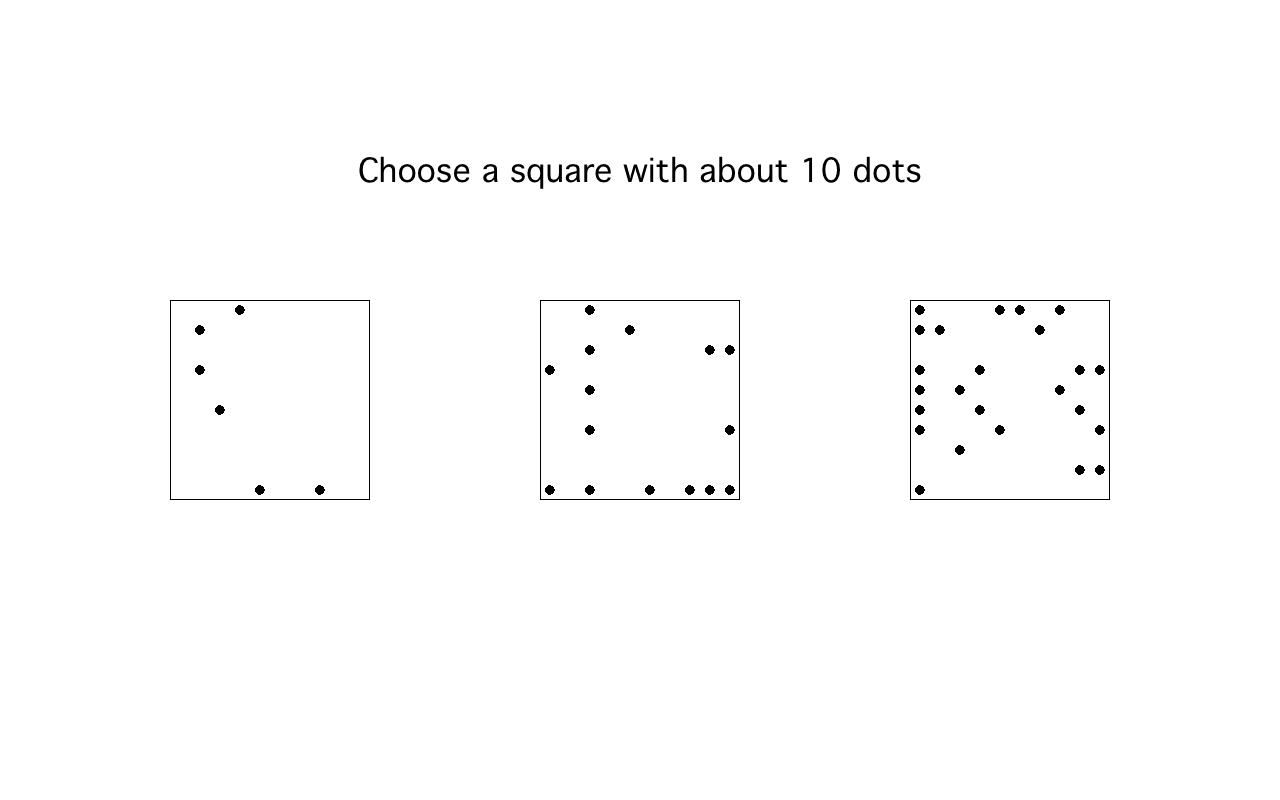
\includegraphics[width=.75\textwidth]{figures/Ce1-example-screenshot}
\caption{Experiment 1 and 2 example stimulus}
\label{Experiment1and2examplestimulus}
\end{figure}

\subsection{Hypotheses (Experiment 1)} 

We formulated the following hypotheses for Experiment 1:

\begin{description}
	\item [Hypothesis 1 (Crisp/Vague RT)] Vague instructions should result in faster responses than crisp instructions; and this pattern should hold when the model is restricted to numeric-only data and when it is restricted to verbal-only data.
	\item [Hypothesis 2 (Numeric/Verbal RT)] There should be no real difference between responses to Numeric instructions and Verbal instructions (based on our interpretation of the experiment in \citet{green2013utility}, where we thought that vague instructions alone were driving the advantage for instructions that were both vague, and also in verbal format).
	\item [Hypothesis 3 (Item RT)] Responses should take longer as the number of dots in the display grows larger (i.e., as the levels of Item increase).
	\item [Hypothesis 4 (Response Type)] Vague instructions should lead to more borderline responses than crisp instructions.
\end{description}

\subsection{Results (Experiment 1)} 

\paragraph{\textbf{Response times}}

30 participants were recruited. Response times from all trials were trimmed at 2.5 standard deviations for each subject, leading to the loss of 236 trials, 3.1\% of the data. The distribution of remaining response times was skewed with many long responses. These remaining response times were log-transformed which reduced this skew so that their distribution more closely approximated a normal distribution. Condition means for response times are given in Figure \ref{resultsC-exp-1-RT}. 

\begin{figure}[htbp]
\centering
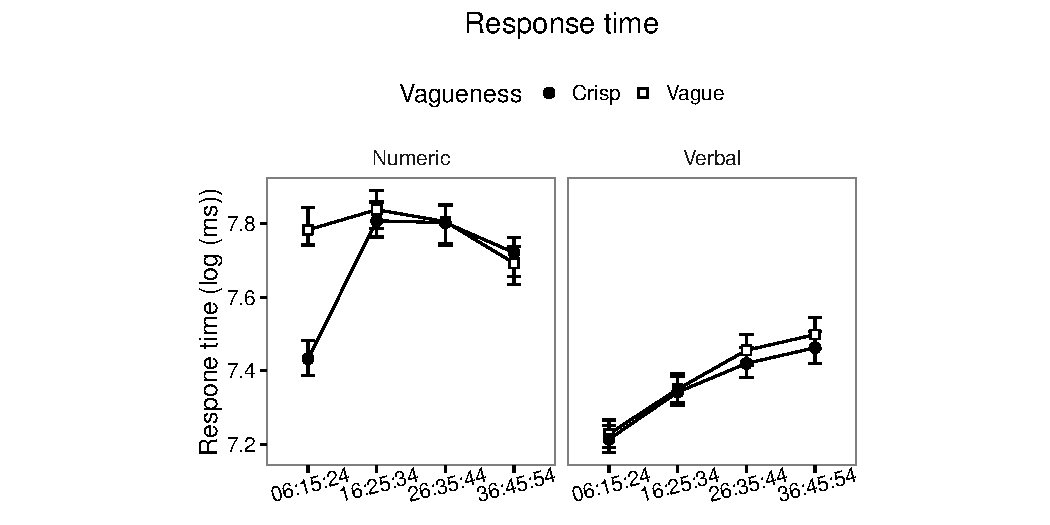
\includegraphics[width=\textwidth]{figures/Ce1-rtplot-1.pdf}
\caption{Experiment 1 results: mean response times by condition and item}
\label{resultsC-exp-1-RT}
\end{figure}

A linear mixed model was constructed for the (log-transformed) response times, with sum-coded vagueness, instruction format, and their interaction, and item, as fixed effects, and per-participant intercepts and slopes for sum-coded vagueness, instruction format, and their interaction as random effects. 

\begin{description}
	\item [Test of Hypothesis 1 (Crisp/Vague RT)] Vague instructions actually led to significantly slower responses than crisp instructions, against Hypothesis 1: $\beta=0.058$, $se=0.013$, $t=4.55$, $p<0.001$. When the model was restricted to numeric-only instructions Vague instructions still led to significantly slower responses than crisp instructions $\beta=0.093$, $se=0.021$, $t=4.51$, $p<0.001$. When the model was restricted to verbal-only instructions Vague instructions tended to slow responses, but not significantly: $\beta=0.024$, $se=0.016$, $t=1.46$, $p=0.155$.
	\item [Test of Hypothesis 2 (Numeric/Verbal RT)] There was actually a significant difference between numeric and verbal instructions, with numeric instructions leading to longer responses than verbal instructions, against Hypothesis 2: $\beta0.265=$, $se=0.072$, $t=5.08$, $p<0.001$.
	\item [Test of Hypothesis 3 (Item RT)] Responses took longer as the levels of Item increased, supporting Hypothesis 3: $\beta=0.120$, $se=0.017$, $t=7.11$, $p<0.001$.
\end{description}

However, given that the response time plot in Figure \ref{resultsC-exp-1-RT} shows that responses to 6:15:24 in the "crisp numeric" instructions condition were extremely fast relative to the "vague numeric" instructions to 6:15:24, the effects in the model of the full dataset could be driven by this difference. A clearer picture of the effects of interest might be obtained by removing the 6:15:24 level of Item from the data set, and fitting the model to this restricted data. Doing this did not affect the direction of the effects in the full dataset, but whereas the effects were significant in the full dataset, they were not significant in the restricted dataset. Full details of the analysis of the restricted dataset are available in the online materials.

\paragraph{\textbf{Borderline cases}}

A generalized linear mixed model \citet{jaeger2008categorical} was fit to the data for the distribution of responses indicating the borderline response, with sum-coded vagueness, instruction format, (and their interaction), and item as fixed effects, and the same effects as slopes over participant, as well as per-participant intercepts as random effects. The distribution of responses over the nearest match square, the borderline square, and the furthest match square are given in Figure \ref{resultsC-exp-1-BL}. Participants chose the borderline square on $16.6\%$ of trials overall.

\begin{figure}[htbp]
\centering
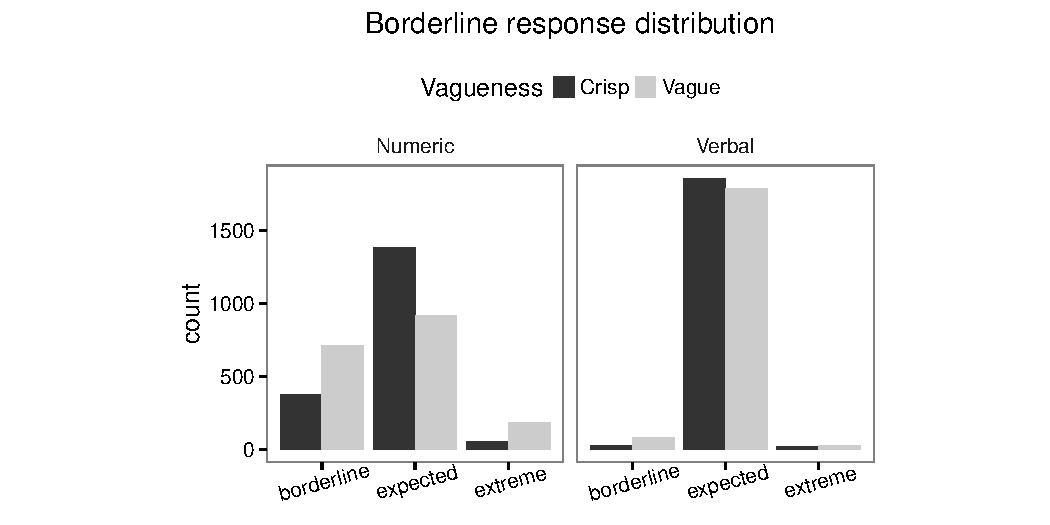
\includegraphics[width=\textwidth]{figures/Ce1-blBarChart-1}
\caption{Experiment 1 results: counts of borderline case responses by condition.}
\label{resultsC-exp-1-BL}
\end{figure}

\begin{description}
	\item [Test of Hypothesis 4 (Response Type)] Participants were significantly more likely to choose the borderline option for vague instructions than for crisp instructions (21.9\% vs 11.3\%: $\beta=0.62$, $se=0.22$, $z=2.8$, $p=0.0059$). Participants were also significantly more likely to choose the borderline square when the instruction used the numerical format rather than the verbal format (30.1\% vs 3.0\%: $\beta=-3.35$, $se=0.23$, $z=-14.6$, $p<0.0001$). 
\end{description}

\subsection{Discussion (Experiment 1)}

This experiment tested whether vague instructions would result in faster responses than crisp instructions, when borderline cases were present. Faster responses for vague instructions were found in pilot experiment B, but there were no borderline cases in that experiment.

In this experiment we found in contrast that vague instructions resulted in slower responses than crisp instructions: a difference that was significant when considering the full data (112ms), but which was not significant after removing the smallest arrays from the analysis, which had a pattern opposite to the main trends in the rest of the data.

We also found that the effect of instruction format was significant, with numerical format slowing responses by 689 ms on average, such that the disadvantage of numerical format overwhelmed the contribution of vagueness. The verbal vague condition still yielded faster responses than the numerical crisp condition, so the pattern from pilot experiment B was reproduced, but in the light of the evidence from this experiment (Experiment 1), in the presence of borderline cases, the advantage that was ascribed to vagueness before now looks more like an advantage of verbal instruction format.

However, once again there is a possibly confounding factor. Observe that, in Experiment 1, instruction format (i.e., the difference between numeric and verbal) went hand in hand with might be called the (human) "selection algorithm": To see this, consider the task of selecting the dot array that contains "few dots":" to do this, it suffices to \emph{compare} the three arrays and select the one that contains the fewest elements.  To select the dot array that contains "16 dots" seems to require the participant to estimate, and then \emph{match}, the cardinality of (at least) one dot array to 16, a process which could plausibly take longer, independently of vagueness. Therefore, our results so far permit the interpretation that what made the instructions in the verbal condition fast is not the fact that they were worded verbally, but that they allowed participants to use \emph{comparison} rather than having to resort to \emph{matching}.

In the next two experiments we pitted the comparison algorithm and matching algorithm selection tasks against each other while controlling vagueness and instruction format. In Experiment 2 we restricted all the instructions to numeric quantifiers while factorially manipulating vagueness and selection task. In Experiment 3 we ensured that all instructions used verbal quantifiers, while also factorially manipulating vagueness and selection task. This allowed us to distinguish between the predictions of the selection task account and the instruction format account. 

\section{Experiment 2: focus on instructions that contain numerals}\label{e2}% D_Exp_2

The main aim of Experiment 2 was to see whether vagueness would exert beneficial effects when all conditions used numerals in the instructions, and when there were vague and crisp versions of the instructions for both comparison and matching strategies. The main changes from Experiment 1 were that the human selection task was explicitly controlled (i.e., whether the task amounted to matching or comparison), and that all conditions were constrained to mention a number. We used the same arrays as in Experiment 1 (an example stimulus is given in Figure \ref{Experiment1and2examplestimulus}). We used a 2 x 2 factorial manipulation of vagueness and selection task (see Table \ref{Instructions for e2}). On each trial an instruction was presented: participants pressed a key to dismiss the instruction, at which time the dot arrays were presented until the participant responded, and the response time and choice were recorded. Table \ref{Instructions for e2} shows the instructions for each condition. Note the difference between ``fewer than 20'' and ``far fewer than 20'': whereas the former cannot have borderline cases (i.e., for each number it is clear whether the number is smaller than 20 or not), the latter can.

\begin{table}
\centering
\caption{Experiment 2: Instructions arranged by condition. The instructions given in the table started with ``Choose a square with \ldots"} 
\label{Instructions for e2}
\begin{tabular}{cccll}
\hline\noalign{\smallskip}
Item & Quantity & Selection & Crisp & Vague \\ 
\noalign{\smallskip}\hline\noalign{\smallskip}
06:15:24 & Small & Comparison & fewer than 20 dots & far fewer than 20 dots \\ 
06:15:24 & Small & Matching & 6 dots & about 10 dots \\ 
06:15:24 & Large & Comparison & more than 10 dots & far more than 10 dots \\ 
06:15:24 & Large & Matching & 24 dots & about 20 dots \\ 
\noalign{\smallskip}\hline\noalign{\smallskip}
16:25:34 & Small & Comparison & fewer than 30 dots & far fewer than 30 dots \\ 
16:25:34 & Small & Matching & 16 dots & about 20 dots \\ 
16:25:34 & Large & Comparison & more than 20 dots & far more than 20 dots \\ 
16:25:34 & Large & Matching & 34 dots & about 30 dots \\ 
\noalign{\smallskip}\hline\noalign{\smallskip}
26:35:44 & Small & Comparison & fewer than 40 dots & far fewer than 40 dots \\ 
26:35:44 & Small & Matching & 26 dots & about 30 dots \\ 
26:35:44 & Large & Comparison & more than 30 dots & far more than 30 dots \\ 
26:35:44 & Large & Matching & 44 dots & about 40 dots \\ 
\noalign{\smallskip}\hline\noalign{\smallskip}
36:45:54 & Small & Comparison & fewer than 50 dots & far fewer than 50 dots \\ 
36:45:54 & Small & Matching & 36 dots & about 40 dots \\ 
36:45:54 & Large & Comparison & more than 40 dots & far more than 40 dots \\ 
36:45:54 & Large & Matching & 54 dots & about 50 dots \\ 
\noalign{\smallskip}\hline
\end{tabular}
\end{table}

\subsection{Hypotheses (Experiment 2)}

For Experiment 2, we formulated the following hypotheses:

\begin{description}
	\item [Hypothesis 1 (Crisp/Vague RT)] Vague instructions should result in faster responses than crisp instructions.
	\item [Hypothesis 2 (Comparison/Matching RT)] Instructions that allow comparison should result in faster responses than instructions that necessitate matching.
	\item [Hypothesis 3 (Interaction)] The vagueness effect should differ according to whether the selection task is comparison or matching.
\end{description}

\subsection{Results (Experiment 2)}

38 participants were recruited. Response times from all trials were trimmed at 2.5 standard deviations for each subject, leading to the loss of 204 trials (2.8\% of the trials). The distribution of remaining response times was skewed with many long responses. These remaining response times were log-transformed which reduced this skew so that their distribution more closely approximated a normal distribution. Condition means for response times are plotted in Figure \ref{resultsD-exp-2}. 

\begin{figure}[htbp]
\centering
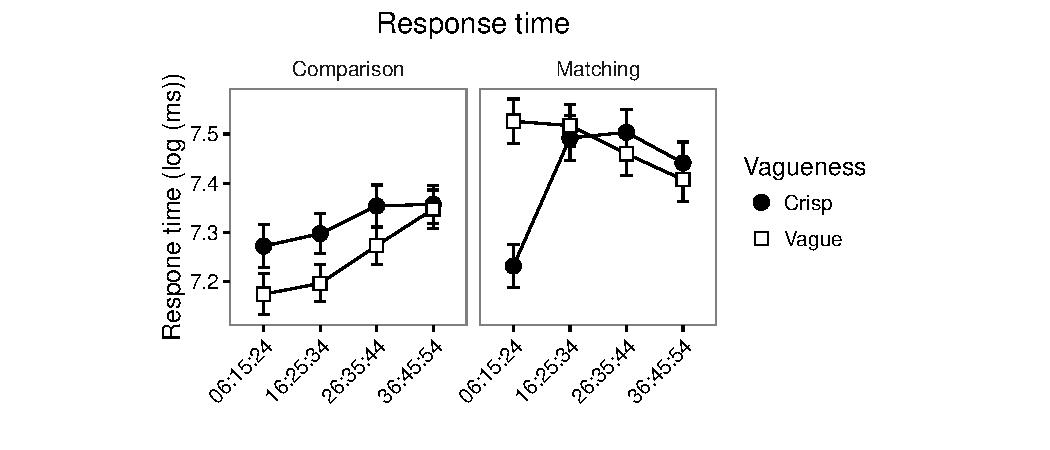
\includegraphics[width=\textwidth]{figures/De2-rtplot-1.pdf}
\caption{Mean response times by condition for Experiment 2 where all instructions were numeric}
\label{resultsD-exp-2}
\end{figure}

A linear mixed model was constructed for the logged response times, with sum-coded vagueness, selection task, and their interaction, and item as fixed effects, and per-participant intercepts and slopes for sum-coded vagueness, selection task, and their interaction, and item for random effects.

\begin{description} 
	\item [Test of Hypothesis 1 (Crisp/Vague RT)] Vague instructions resulted in faster responses than crisp instructions on average. However this difference was not significant in the full model ($\beta=-0.0057$, $se=0.0137$, $t=-0.42$, $p=0.678$). Using Levy's method \citep{Levy:MainEffectsInteractions} to test for main effects in the presence of higher-order interactions, by doing model comparison between a null model that included all interaction terms involving Vagueness but leaving out a term for the main effect of Vagueness, against a full model that differed only by including Vagueness as a main effect, showed that the full model was no better than the reduced model ($df=1$, $p=0.676$), consituting more evidence that Vagueness did not exert a significant main effect on response times. 
	\item [Test of Hypothesis 2 (Comparison/Matching RT)] comparison instructions resulted in faster responses than matching instructions, and the difference was significant ($\beta=0.1618$, $se=0.0255$, $t=6.34$, $p<0.001$).
	\item [Test of Hypothesis 3 (Interaction)] Although Vagueness did not exert a significant main effect, Vagueness did exert effects in interactions with some other variables: the interaction between Vagueness and Selection task  was significant ($\beta=0.1306$, $se=0.0205$, $t=6.38$, $p<0.001$), suggesting that Vagueness speeded RTs in the comparison condition but slowed them down in the matching task. 
\end{description}

\subsection{Discussion (Experiment 2)}

The cost reduction account predicted that there should be a significant main effect of Vagueness such that responses would be faster for Vague intructions than for crisp instructions. We found that although there was a very small effect in that direction, the effect was not statistically significant. Models that differed only in the presence of Vagueness as a main effect were shown not to differ significantly in their explanatory value. However we did find that Vagueness exerted effects on other variables: Vagueness speeded RTs in the comparison task and slowed RTs in the matching task.

\section{Experiment 3: focus on instructions that do not contain numerals}\label{e3}\marginnote{E-Exp-3}

This experiment mirrors Experiment 2, but focussing on instructions that did not use a number. We manipulated vagueness and the selection task (comparison and matching). In order to implement the experiment without mentioning numbers in the instructions, we changed the sequence of each trial to include a `target' (i.e., a dot array of a particular cardinality) before the array, so that we could then refer to the target's cardinality in the instruction using expressions like \emph{the same number of dots as the target}; \emph{fewer dots than the target}. An example of this sequence is given in Figure \ref{Experiment3examplestimulus}. This presentation of a target before the main body of the trial shares some features with \citeauthor[Experiment 2]{Izard20081221}, although in that experiment participants were told the cardinality of the target (called an \emph{inducer} in that paper) whereas in our experiment we did not tell participants the cardinality of the prime array. An item was thus a combination of a target dot array, an instruction that did not contain a number, and a set of dot arrays taking their cardinalities from the same triples used in Experiments 1 and 2. Table \ref{instructionsE-exp-3} spells out how the instructions were constrained not to mention a numeral and gives examples of targets.

\begin{figure}[htbp]
\centering
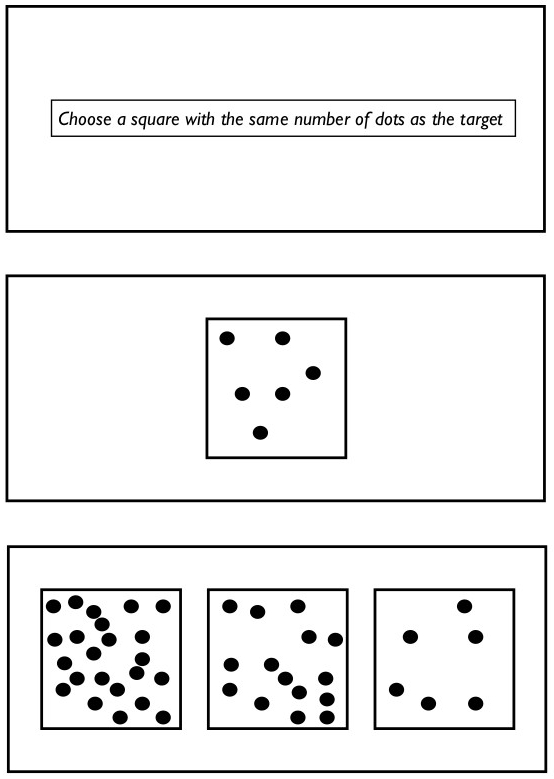
\includegraphics[width=.75\textwidth]{figures/Ee3-flow.jpg}
\caption{Experiment 3 example stimulus}
\label{Experiment3examplestimulus}
\end{figure}

\begin{table}
\centering
\caption{Experiment 3 instructions arranged by condition. The instructions given in the table started with ``Choose a square with \ldots"}
\label{instructionsE-exp-3}
\resizebox{\textwidth}{!}{\begin{tabular}{ccccll}
\hline\noalign{\smallskip}
Item & Target & Quantity & Selection & Crisp & Vague \\ 
\noalign{\smallskip}\hline\noalign{\smallskip}
06:15:24 &   6 & Small & Matching 	& the same number of dots as the target & NA \\ 
06:15:24 &  10 & Small & Matching 	& NA & about the same number of dots as the target \\ 
06:15:24 &  10 & Large & Comparison & more dots than the target & far more dots than the target \\ 
06:15:24 &  20 & Small & Comparison & fewer dots than the target & far fewer dots than the target \\ 
06:15:24 &  20 & Large & Matching 	& NA & about the same number of dots as the target \\ 
06:15:24 &  24 & Large & Matching 	& the same number of dots as the target & NA \\ 
\noalign{\smallskip}\hline\noalign{\smallskip}
16:25:34 &  16 & Small & Matching 	& the same number of dots as the target & NA \\ 
16:25:34 &  20 & Small & Matching 	& NA & about the same number of dots as the target \\ 
16:25:34 &  20 & Large & Comparison & more dots than the target & far more dots than the target \\ 
16:25:34 &  30 & Small & Comparison & fewer dots than the target & far fewer dots than the target \\ 
16:25:34 &  30 & Large & Matching 	& NA & about the same number of dots as the target \\ 
16:25:34 &  34 & Large & Matching 	& the same number of dots as the target & NA \\ 
\noalign{\smallskip}\hline\noalign{\smallskip}
26:35:44 &  26 & Small & Matching 	& the same number of dots as the target & NA \\ 
26:35:44 &  30 & Small & Matching 	& NA & about the same number of dots as the target \\ 
26:35:44 &  30 & Large & Comparison & more dots than the target & far more dots than the target \\ 
26:35:44 &  40 & Small & Comparison & fewer dots than the target & far fewer dots than the target \\ 
26:35:44 &  40 & Large & Matching 	& NA & about the same number of dots as the target \\ 
26:35:44 &  44 & Large & Matching 	& the same number of dots as the target & NA \\ 
\noalign{\smallskip}\hline\noalign{\smallskip}
36:45:54 &  36 & Small & Matching 	& the same number of dots as the target & NA \\ 
36:45:54 &  40 & Small & Matching 	& NA & about the same number of dots as the target \\ 
36:45:54 &  40 & Large & Comparison & more dots than the target & far more dots than the target \\ 
36:45:54 &  50 & Small & Comparison & fewer dots than the target & far fewer dots than the target \\ 
36:45:54 &  50 & Large & Matching 	& NA & about the same number of dots as the target \\ 
36:45:54 &  54 & Large & Matching 	& the same number of dots as the target & NA \\ 
\noalign{\smallskip}\hline
\end{tabular}}
\end{table}

\subsection{Hypotheses}

For Experiment 3, we hypothesised:

\begin{description}
	\item [Hypothesis 1] Vague instructions are easier for the reader than crisp ones (main effect of vagueness)
	\item [Hypothesis 2] Comparison is easier for the reader than matching (main effect of selection)
	\item [Hypothesis 3] Effects of vagueness differ depending on whether selection is matching or comparison (interaction effect selection x vagueness, and focussed comparisons at each level of selection).
\end{description}

\subsection{Results}
40 volunteers participated. The results showed that vagueness was beneficial for comparison but detrimental for matching (the same as Experiment 2) even when no numbers were allowed in the instructions. Figure \ref{resultsE-exp-3} shows the means by condition. Our findings were as follows:

\begin{description}
	\item [Test of hypothesis 1] There was no significant main effect of vagueness ($\beta=-0.02$, $se=0.01$, $t=-1.5$, $p=0.1296$). 
	\item [Test of hypothesis 2] There was a main effect of selection, with comparison task instructions leading to faster responses than the matching task instructions ($\beta=0.18$, $se=0.02$, $t=10.4$, $p<0.0001$).  This effect was in the same direction as Experiment 3. 
	\item [Test of hypothesis 3] Vagueness did exert different effects depending on the selection task (main interaction effect of vagueness by selection $\beta=0.12$, $se=0.02$, $t=5.1$, $p<0.0001$). 
Separate analyses of the effect of vagueness were conducted for the comparison task and for the matching task using Bonferroni-adjusted significance thresholds. 
In the comparison task, vagueness resulted in faster response times ($\beta=-0.08$, $se=0.02$, $t=-4.3$, $p<0.0001$). 
In the matching task vagueness slowed response times ($\beta=0.05$, $se=0.01$, $t=3.7$, $p=0.0004$). 
These results are in the same direction as Experiment 3.
\end{description}

Once again, the cost reduction account was wrong to predict main effect advantages for vagueness, and wrong to predict that vagueness should be beneficial at each level of the selection task: however vagueness was advantageous in the comparison task.

\begin{figure}[htbp]
\centering
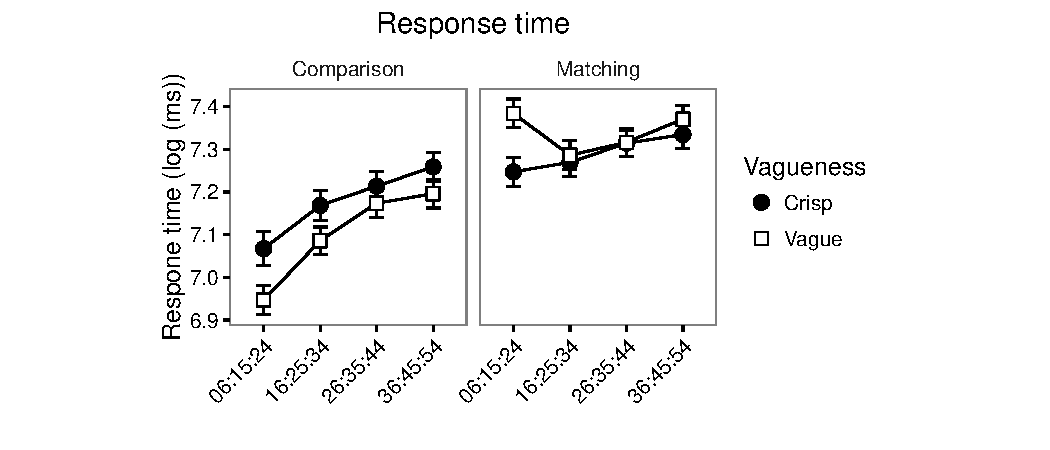
\includegraphics[width=\textwidth]{figures/Ee3-rtplot-1.pdf}
\caption{Mean response times by condition for Experiment 3}
\label{resultsE-exp-3}
\end{figure}

\section{Discussion of experiments 2 and 3}\label{discussion-of-e2-and-e3}The main aim of these two experiments was to test whether vagueness confers any cognitive benefits over and above those due to differences in the selection task according to whether the instruction mandates a \emph{comparison} selection task or a \emph{matching} selection task, when number-use is held constant. The main effect of selection task showed that the assumption that the \emph{comparison} task is easier than the \emph{matching} task is well-founded. In both experiments people were reliably quicker to respond in the \emph{comparison} task. 

Vagueness, which was the phenomenon on which our investigation focussed, did not exert a significant main effect in response time. However when the comparison and selection tasks were analysed separately, there was small significant advantage for vagueness in the \emph{comparison} tasks, but a small significant disadvantage for vagueness in the \emph{matching} tasks. 

\section{General Discussion}\label{general-discussion}To summarise our findings, we asked why strategic vagueness is as frequent as it is and we decided to focus on what we see as the most promising explanation, namely that vague expressions are easy to process by speakers and hearers: the cost hypothesis, as we have called it. We decided to test this hypothesis by experimentally investigating whether vague descriptions are resolved by hearers more quickly than crisp ones. Although we were able to find some interesting (and statistically highly significant) effects, it appears to us that if our sequence of experiments is assessed as a whole, it cannot be seen as confirmation of the cost hypothesis.

To explain why this is, let us summarise our findings so far: %
%\citet{green2013utility} showed that responses were faster and more accurate when the instructions were vague than when they were crisp, but the experiment was unable to distinguish effects of vagueness from those of number-avoidance or selection task: the vague conditions were also in verbal rather than numerical format, and they mandated a comparison strategy rather than a matching strategy. 
%
Experiment 1 showed that number avoidance in the verbal format instructions is an important factor driving the faster response times in the task, and that vagueness does not have any additional benefit in either the verbal format instructions or the numerical format instructions. However, Experiment 1 did not distinguish benefits of number avoidance from benefits of the comparison selection task. In Experiments 2 and 3 we manipulated vagueness and the selection task, separately at each level of numerical format. Across the two experiments, we found that the comparison-task instructions attracted faster response times than the matching-task instructions. Within the two experiments we found that vagueness exerts benefits when the selection task is \emph{comparison}, but not when the task is \emph{matching}.

What is one entitled to conclude? Given that we were able to identify a class of situations in which vague expressions led to faster response times than crisp ones, would it be valid to conclude that we have finally discovered an advantage for vagueness that cannot be ascribed to some other factor? We believe the answer to this question is negative.

\begin{table}[htbp]
\caption{Vagueness as range reduction: a summary of Experiments 2 and 3}
\label{Vagueness as range reduction}
\centering
\begin{tabular}{cccc}
\hline\noalign{\smallskip}
selection task 					& vagueness		& candidates	& effect of vagueness						\\
\noalign{\smallskip}\hline\noalign{\smallskip}
\multirow{ 2}{*}{comparison} 	& crisp 		& 2				& \multirow{ 2}{*}{vagueness advantage}  	\\
\noalign{\smallskip}\cline{2-3}\noalign{\smallskip}
								& vague			& 1				&                                           \\
\noalign{\smallskip}\hline\noalign{\smallskip}
\multirow{ 2}{*}{matching} 		& crisp 		& 1 			& \multirow{ 2}{*}{vagueness disadvantage}	\\
\noalign{\smallskip}\cline{2-3}\noalign{\smallskip}
								& vague			& 2				&								 			\\
\noalign{\smallskip}\hline
\end{tabular}
\end{table}

To see why, consider Figures \ref{resultsD-exp-2} and \ref{resultsE-exp-3}. Both figures depict four conditions, depending on whether the expression was crisp or vague, and depending on whether the referent could be identified using a comparison strategy or not. Two of the resulting four conditions result in an expression that can denote either of two referents; the other two conditions result in an expression that can only denote one referent, with the other possible referent being a marginal candidate at best.

To see why vagueness has opposite effects, depending on whether it is used in matching or comparison situations, consider the stimulus with (6,15,24) dots. Now compare `Choose a square with 6 dots' with its vague counterpart `Choose a square with about 10 dots': by adding the word `about', we broaden the range of squares that the expression might be referring to. On the other hand, compare `Choose a square with fewer than 20 dots' with `Choose a square with far fewer than 20 dots': by adding the word `far', we did not broaden the range of squares denotable by the expression: we narrow it down, because only some of the squares that have fewer dots may have {\em far} fewer dots.

The benefits of vagueness in the \emph{comparison} task in experiments 3 and 4 could thus be explained as differences in the number of valid targets for the expression. This leads us to speculate that the benefit for vagueness here could be due to the vague expression foregrounding a particular valid target while the crisp expression carries with it the additional task of distinguishing between two alternative valid targets, something we propose to call a ``range-reduction'' benefit.

The observation that conditions with 1 candidate lead to shorter response times than conditions with 2 candidates is consistent with the range reduction hypothesis, but not with the idea that vagueness is beneficial. It appears, in other words, that shorter response times will only result from a vague expression if this expression leads to range reduction. Once again, it is not vagueness itself that has advantages but a phenomenon (namely range reduction) that is an automatic concomitant of vagueness in some types of situations.\\[2ex]
%
\noindent Looking at the entire series of experiments, our findings suggest that the observed benefits of vague expressions may be due to factors other than vagueness: factors like avoiding numbers; permitting comparison tasks; and range reduction. The picture that is starting to emerge is subtle: on the one hand, in the situations that we have been studying vagueness is not intrinsically beneficial. On the other hand, vague expressions frequently possess other features that \emph{are} beneficial, and these are what give us the incorrect impression that vagueness itself is beneficial. Vagueness may thus have acquired a reputation that it does not deserve. The answer to Lipman's question, of why vagueness permeates human language (see our Introduction), may lie in a different direction after all, possibly relating to benefits for the speaker rather than the hearer.

A comparison may clarify the logic of the situation. In recent years a number of studies, focussing on red wine, have suggested that alcohol, consumed in low doses, may have health benefits. An alternative explanation, however, asserts that it is not the alcohol in the wine that was beneficial, but antioxidants from grapes. If this alternative explanation is correct, then alcohol may not be healthy after all.\\[2ex]
%
% KvD Feb 2017. I've diminished the role of NLG in the coming paragraph.
Our findings suggest a re-think of the questions on which much research on the utility of vagueness rests. Years of research on the logic of vagueness -- giving rise to such techniques as Partial Logic \citep[e.g.,][]{Fine}, Probabilistic Logic \citep{Edgington}, and Fuzzy Logic \citep{Zadeh} -- have primed the research community to expect that some special utility of vagueness is an important part of the answer, but our findings call this expectation into question. 

Although our own studies in this article have focussed on vagueness in descriptive Noun Phrases only, it seems to us plausible that vagueness plays a similar role in other
linguistic constructs. For example, consider reports on air temperature. Given a numerical
temperature measurement or prediction, we might word it as 
%
\begin{quote}
(a) {\em 27.2 degrees Celsius}, or\\
(b) {\em approximately 27 degrees}, or\\
(c) {\em above 25 degrees}, or\\
(d) {\em warm}, 
\end{quote}
%
among other candidate expressions. Which of these descriptions is most effective, for example as part of a weather report? If the linguistic literature is to be believed, then options (a) and (c) convey crisp information, whereas (b) and (d) are vague (i.e., they permit borderline cases). In the situations studied in our own experiments and the ones discussed in section 1, we found no evidence that vagueness is beneficial for hearers. Rather than asking whether a candidate expression is vague, other questions might shed more light on the choice, similar to the ones identified in our studies. These questions might focus on the amount of information that a given expression conveys (i.e., on granularity), on the avoidance of numbers, and on the use of evaluative terms. Let's see how this might pan out for the above examples from the weather domain.

First, the experiments by \citeauthor{Mishra01042011} suggest that it is important how much information is conveyed by an expression, and their findings are echoed by our own thoughts about range reduction (following Experiments 2 and 3). In the case of (a)--(d) above, it appears that (a) conveys the most detailed information (designating the smallest segment of the temperature scale), followed by (b), then (d), then (c) (e.g., 40 degrees is above 25, but at 40 Celsius the word ``warm'' is likely to give way to ``hot'' or ``scorching''): 
%
\begin{quote}
$a < b < d < c$
\end{quote}
%
If these hunches are correct, then it seems to us that it is relatively unimportant whether a given expression is vague or crisp. Other factors seem more important; moreover, it may depend on the task and the audience which of a-d is preferred. For example, an \emph{expert} may prefer to read expression (a), because it gives her the most detailed information on which to base her decisions. On the other hand, expression (d) (``warm'') is shorter than the other three and avoids the use of numbers; our experiments suggest that this may make (d) more rapidly understood than its competitors; earlier experiments point in the same direction, given the evaluative nature of ``warm'' (recall our section 1.2), which is especially important if the hearer is unfamiliar with the metric used. These considerations suggest that {\em non-experts} might prefer expression (d). 

One way to see why vagueness (as defined in our Introduction) may not benefit human communication is the following thought experiment. Suppose a group of speakers understand the word ``warm'' as vague, agreeing that temperatures above 26 count as warm, and temperatures below 24 do not count as warm, but considering temperatures between 24 and 26 as borderline cases. Now one day these speakers agree to sharpen up their definition deciding that, henceforth, ``warm'' means ``$>25$ degrees'' (as in (c) above): this decision resolves the borderline cases, while everything else remains the same. It seems unlikely that this change in language use, from a vague meaning to a crisp one (i.e., one that has no borderline cases anymore), would lower the utility of the word. Our experimental findings,
and the conclusions that we draw from them, are consistent with this idea.

\backmatter
\bibliographystyle{spbasic}
\bibliography{v-book-2018}
\backmatter
%\printindex
\end{document}
